% Options for packages loaded elsewhere
\PassOptionsToPackage{unicode}{hyperref}
\PassOptionsToPackage{hyphens}{url}
%
\documentclass[
  ignorenonframetext,
]{beamer}
\usepackage{pgfpages}
\setbeamertemplate{caption}[numbered]
\setbeamertemplate{caption label separator}{: }
\setbeamercolor{caption name}{fg=normal text.fg}
\beamertemplatenavigationsymbolsempty
% Prevent slide breaks in the middle of a paragraph
\widowpenalties 1 10000
\raggedbottom
\setbeamertemplate{part page}{
  \centering
  \begin{beamercolorbox}[sep=16pt,center]{part title}
    \usebeamerfont{part title}\insertpart\par
  \end{beamercolorbox}
}
\setbeamertemplate{section page}{
  \centering
  \begin{beamercolorbox}[sep=12pt,center]{part title}
    \usebeamerfont{section title}\insertsection\par
  \end{beamercolorbox}
}
\setbeamertemplate{subsection page}{
  \centering
  \begin{beamercolorbox}[sep=8pt,center]{part title}
    \usebeamerfont{subsection title}\insertsubsection\par
  \end{beamercolorbox}
}
\AtBeginPart{
  \frame{\partpage}
}
\AtBeginSection{
  \ifbibliography
  \else
    \frame{\sectionpage}
  \fi
}
\AtBeginSubsection{
  \frame{\subsectionpage}
}
\usepackage{amsmath,amssymb}
\usepackage{lmodern}
\usepackage{iftex}
\ifPDFTeX
  \usepackage[T1]{fontenc}
  \usepackage[utf8]{inputenc}
  \usepackage{textcomp} % provide euro and other symbols
\else % if luatex or xetex
  \usepackage{unicode-math}
  \defaultfontfeatures{Scale=MatchLowercase}
  \defaultfontfeatures[\rmfamily]{Ligatures=TeX,Scale=1}
\fi
\usetheme[]{CambridgeUS}
\usecolortheme{beaver}
\usefonttheme{serif}
% Use upquote if available, for straight quotes in verbatim environments
\IfFileExists{upquote.sty}{\usepackage{upquote}}{}
\IfFileExists{microtype.sty}{% use microtype if available
  \usepackage[]{microtype}
  \UseMicrotypeSet[protrusion]{basicmath} % disable protrusion for tt fonts
}{}
\makeatletter
\@ifundefined{KOMAClassName}{% if non-KOMA class
  \IfFileExists{parskip.sty}{%
    \usepackage{parskip}
  }{% else
    \setlength{\parindent}{0pt}
    \setlength{\parskip}{6pt plus 2pt minus 1pt}}
}{% if KOMA class
  \KOMAoptions{parskip=half}}
\makeatother
\usepackage{xcolor}
\IfFileExists{xurl.sty}{\usepackage{xurl}}{} % add URL line breaks if available
\IfFileExists{bookmark.sty}{\usepackage{bookmark}}{\usepackage{hyperref}}
\hypersetup{
  pdftitle={03-bis - 
aTeX bis},
  hidelinks,
  pdfcreator={LaTeX via pandoc}}
\urlstyle{same} % disable monospaced font for URLs
\newif\ifbibliography
\usepackage{color}
\usepackage{fancyvrb}
\newcommand{\VerbBar}{|}
\newcommand{\VERB}{\Verb[commandchars=\\\{\}]}
\DefineVerbatimEnvironment{Highlighting}{Verbatim}{commandchars=\\\{\}}
% Add ',fontsize=\small' for more characters per line
\newenvironment{Shaded}{}{}
\newcommand{\AlertTok}[1]{\textcolor[rgb]{1.00,0.00,0.00}{#1}}
\newcommand{\AnnotationTok}[1]{\textcolor[rgb]{0.00,0.50,0.00}{#1}}
\newcommand{\AttributeTok}[1]{#1}
\newcommand{\BaseNTok}[1]{#1}
\newcommand{\BuiltInTok}[1]{#1}
\newcommand{\CharTok}[1]{\textcolor[rgb]{0.00,0.50,0.50}{#1}}
\newcommand{\CommentTok}[1]{\textcolor[rgb]{0.00,0.50,0.00}{#1}}
\newcommand{\CommentVarTok}[1]{\textcolor[rgb]{0.00,0.50,0.00}{#1}}
\newcommand{\ConstantTok}[1]{#1}
\newcommand{\ControlFlowTok}[1]{\textcolor[rgb]{0.00,0.00,1.00}{#1}}
\newcommand{\DataTypeTok}[1]{#1}
\newcommand{\DecValTok}[1]{#1}
\newcommand{\DocumentationTok}[1]{\textcolor[rgb]{0.00,0.50,0.00}{#1}}
\newcommand{\ErrorTok}[1]{\textcolor[rgb]{1.00,0.00,0.00}{\textbf{#1}}}
\newcommand{\ExtensionTok}[1]{#1}
\newcommand{\FloatTok}[1]{#1}
\newcommand{\FunctionTok}[1]{#1}
\newcommand{\ImportTok}[1]{#1}
\newcommand{\InformationTok}[1]{\textcolor[rgb]{0.00,0.50,0.00}{#1}}
\newcommand{\KeywordTok}[1]{\textcolor[rgb]{0.00,0.00,1.00}{#1}}
\newcommand{\NormalTok}[1]{#1}
\newcommand{\OperatorTok}[1]{#1}
\newcommand{\OtherTok}[1]{\textcolor[rgb]{1.00,0.25,0.00}{#1}}
\newcommand{\PreprocessorTok}[1]{\textcolor[rgb]{1.00,0.25,0.00}{#1}}
\newcommand{\RegionMarkerTok}[1]{#1}
\newcommand{\SpecialCharTok}[1]{\textcolor[rgb]{0.00,0.50,0.50}{#1}}
\newcommand{\SpecialStringTok}[1]{\textcolor[rgb]{0.00,0.50,0.50}{#1}}
\newcommand{\StringTok}[1]{\textcolor[rgb]{0.00,0.50,0.50}{#1}}
\newcommand{\VariableTok}[1]{#1}
\newcommand{\VerbatimStringTok}[1]{\textcolor[rgb]{0.00,0.50,0.50}{#1}}
\newcommand{\WarningTok}[1]{\textcolor[rgb]{0.00,0.50,0.00}{\textbf{#1}}}
\setlength{\emergencystretch}{3em} % prevent overfull lines
\providecommand{\tightlist}{%
  \setlength{\itemsep}{0pt}\setlength{\parskip}{0pt}}
\setcounter{secnumdepth}{-\maxdimen} % remove section numbering
\AtBeginDocument{\title[\LaTeX bis]{03-bis - \LaTeX bis}}
\usepackage{graphicx}
\usepackage{setspace}
\usepackage{tabularx}
\usepackage[italian]{babel}
\usepackage{tikzsymbols}
\usepackage{subcaption}
\usepackage{tikz}
\usepackage{spot}
\usepackage{tabularx}
\usepackage[absolute,overlay]{textpos}
\usepackage{booktabs}
\newcommand\Factor{1.2}
\setbeamerfont{subtitle}{size=\large, series=\bfseries}
\definecolor{template}{RGB}{54, 114, 89}
\setbeamercolor{frametitle}{bg=white}
\setbeamertemplate{frametitle}[default][center]
\AtBeginSection{\frame{\sectionpage}}
\setbeamercolor{section name}{fg=white}
\ifLuaTeX
  \usepackage{selnolig}  % disable illegal ligatures
\fi

\title{03-bis - 
aTeX bis}
\author{Ottavia M. Epifania\\
University of Padova}
\date{Corso \texttt{RMarkdown}}
\institute{\href{mailto:ottavia.epifania@unipd.it}{\nolinkurl{ottavia.epifania@unipd.it}}}

\begin{document}
\frame{\titlepage}

\begin{frame}{Il perché di questa lezione}
\protect\hypertarget{il-perchuxe9-di-questa-lezione}{}
Quando ho preparato le slide per \LaTeX usando Sweave, tutto sembrava
andare per il meglio

\pause

Poi, gli aggiornamenti e:

\begin{center}
\includegraphics[width=0.5\linewidth]{img/meme} \end{center}
\end{frame}

\begin{frame}[fragile]{}
\protect\hypertarget{section}{}
\begin{itemize}
\item
  \texttt{Sweave} vi obbliga a usare \LaTeX
\item
  Non è facile farlo funzionare, specie se volete aggiungere dei pezzi
  di codice e i risultati delle vostre analisi
\item
  Per usare \texttt{Sweave}, tanto vale usare direttamente \LaTeX
\item
  Vi lascio comunque le
  \href{https://ottaviae.github.io/CorsoRmarkdown/slides/03\%20-\%20LaTeX/03-LaTeX.pdf}{\textcolor{blue}{slide}}
  per conoscenza generale
\end{itemize}
\end{frame}

\begin{frame}{}
\protect\hypertarget{section-1}{}
I file si aprono esattamente come prima. L'unica cosa che modifichiamo è
lo YAML

\begin{exampleblock}{Vantaggi}

\begin{itemize}
\item
  Permette di usare \LaTeX senza realmente saper usare \LaTeX
\item
  Ha tutta la flessibilità (e bellezza) dei file \LaTeX
\item
  Con un minimo sforzo si ottengono dei risultati di tutto rispetto
\end{itemize}

\end{exampleblock}

\pause

\vspace{5mm}

\begin{alertblock}{Svantaggi}

\begin{itemize}
\item
  Se vogliamo ottenere un \texttt{HTML} non è la soluzione che fa per
  noi
\item
  Essendo un ibrido tra \texttt{RMarkdown} e \LaTeX bisogna fare
  attenzione a come comunicano
\item
  Le soluzioni che vanno bene in \LaTeX non sempre vanno bene in
  \texttt{RMarkdown}
\end{itemize}

\end{alertblock}
\end{frame}

\hypertarget{documenti-di-testo}{%
\section{Documenti di testo}\label{documenti-di-testo}}

\begin{frame}{Lo YAML}
\protect\hypertarget{lo-yaml}{}
\begin{center}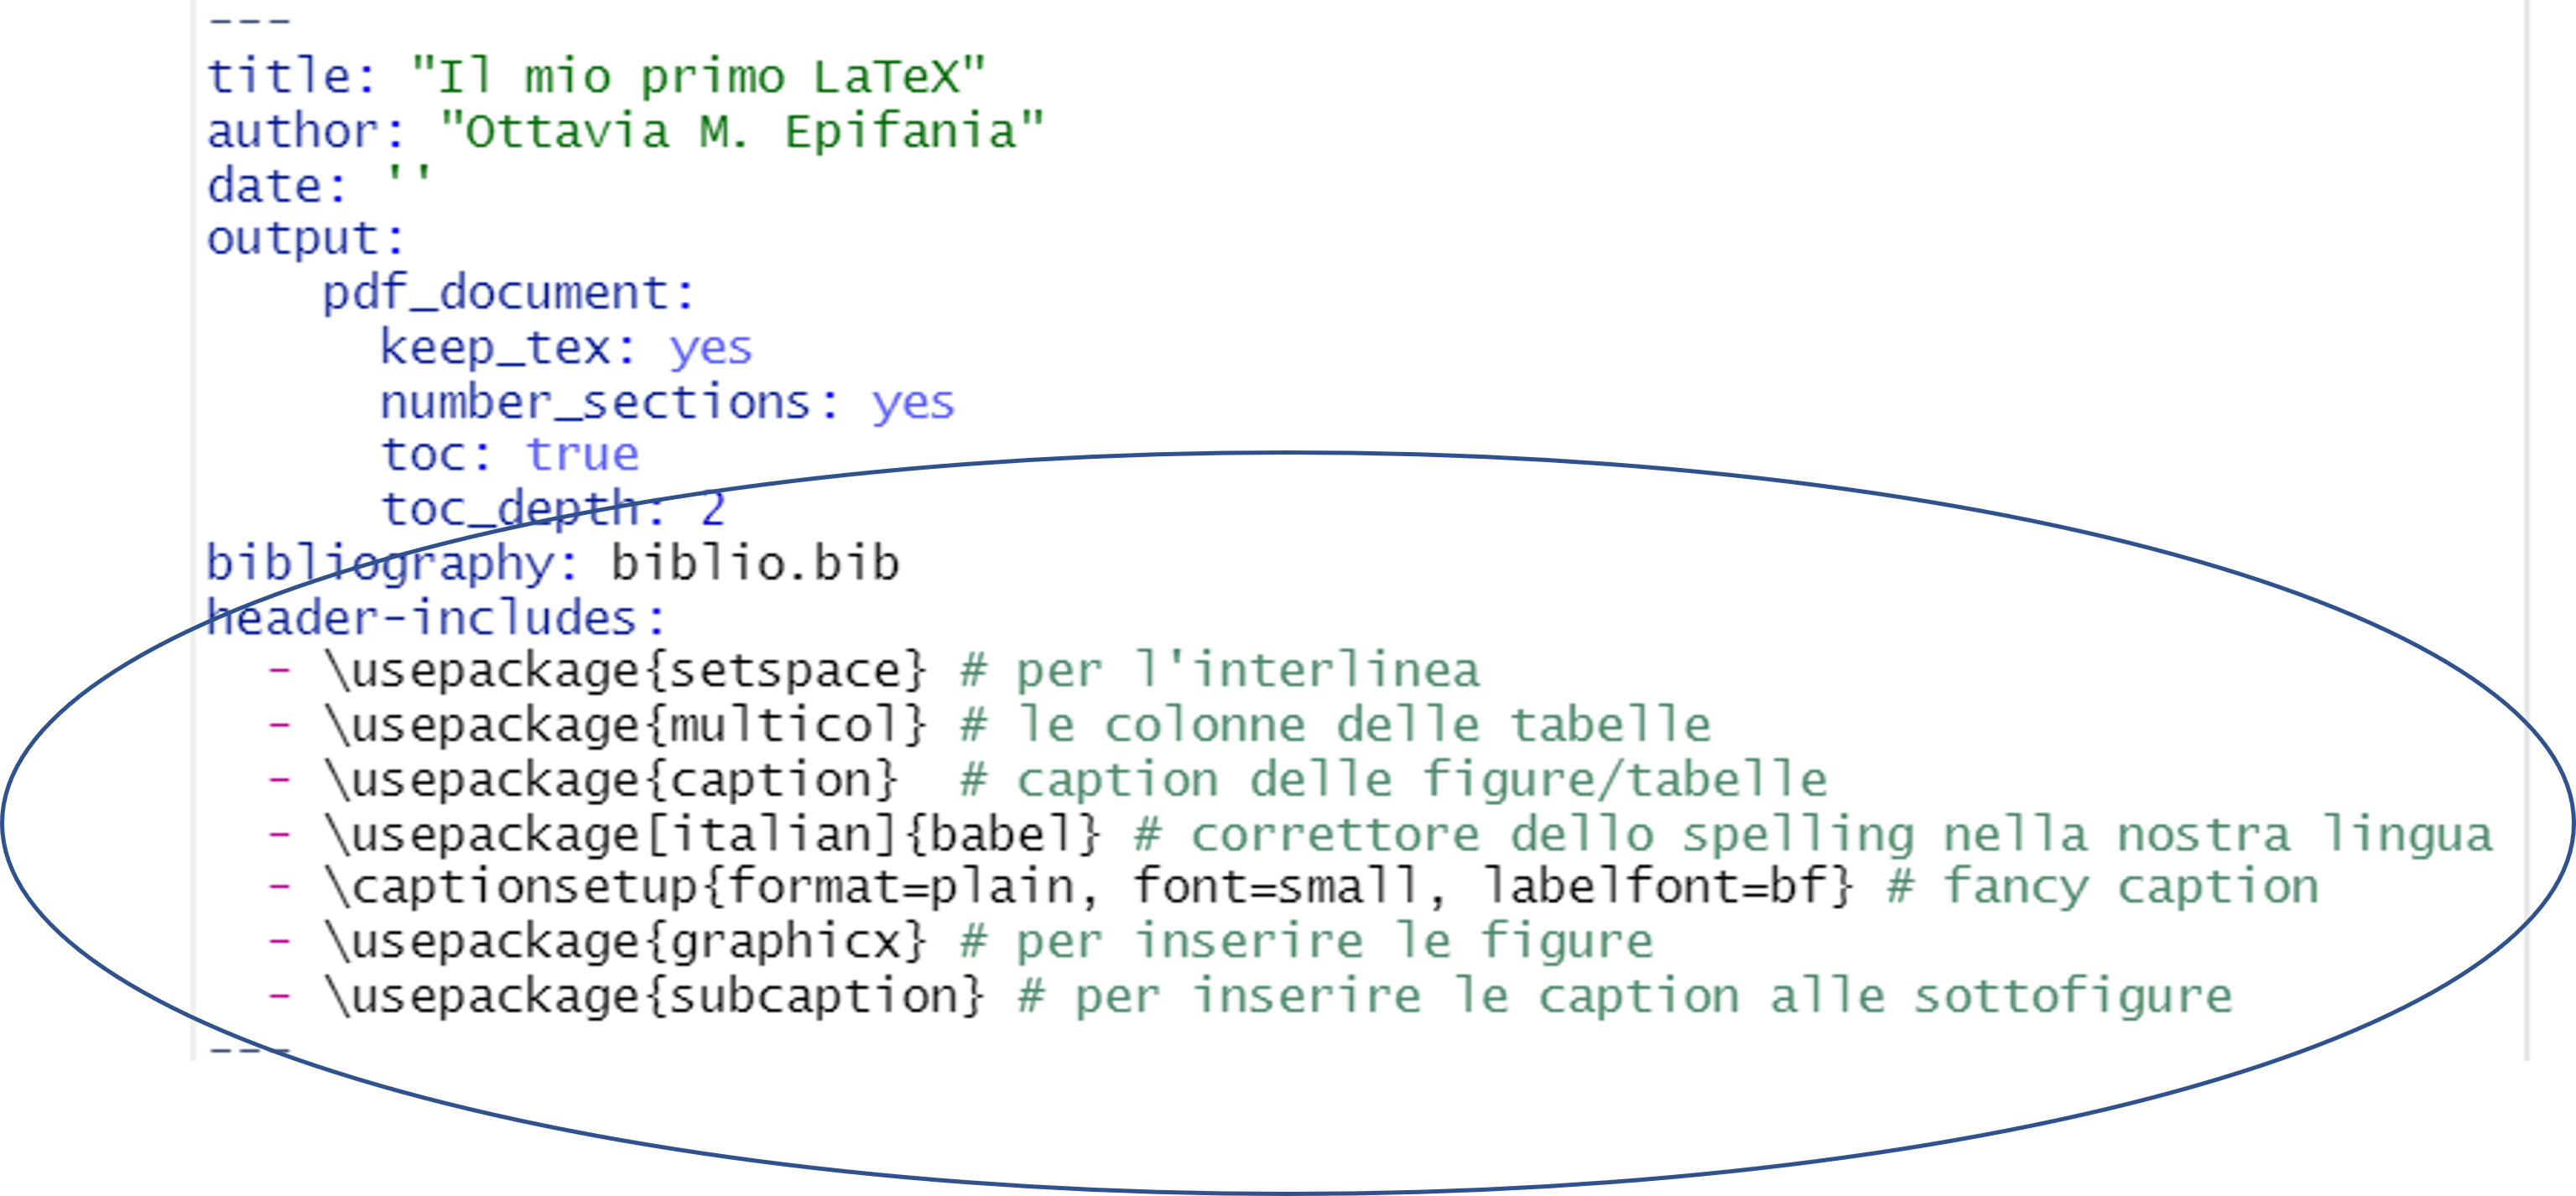
\includegraphics[width=1\linewidth]{img/yaml} \end{center}
\end{frame}

\begin{frame}[fragile]{}
\protect\hypertarget{section-2}{}
Uno YAML come quello di cui sopra vi restituisce un risultato simile a
quello che abbiamo visto fino ad adesso.

Le aggiunte che abbiamo messo ci permettono di utilizzare il file in
maniera più ``elastica'', ossia usando la sintassi e le potenzalità di
\LaTeX ma rimandendo con la logica di \texttt{RMarkdown}
\end{frame}

\begin{frame}[fragile]{Le figure}
\protect\hypertarget{le-figure}{}
Ormai sappiamo a memoria come mettere le figure:

\begin{verbatim}
```{r, out.width="50%"}
knitr::include_graphics(path = "percorso-alla-figura/figura.png")
```
\end{verbatim}

Però abbiamo visto il disagio che è mettere le cross-references con
\texttt{bookdown}

Con \LaTeX invece è molto più semplice, anche se dobbiamo scrivere molto
di più

Bisogna assicurarsi di aggiungere allo YAML:

\begin{Shaded}
\begin{Highlighting}[]
\NormalTok{\textgreater{} {-} }\BuiltInTok{\textbackslash{}usepackage}\NormalTok{\{}\ExtensionTok{graphicx}\NormalTok{\} }
\end{Highlighting}
\end{Shaded}
\end{frame}

\begin{frame}{Codice}
\protect\hypertarget{codice}{}
\begin{center}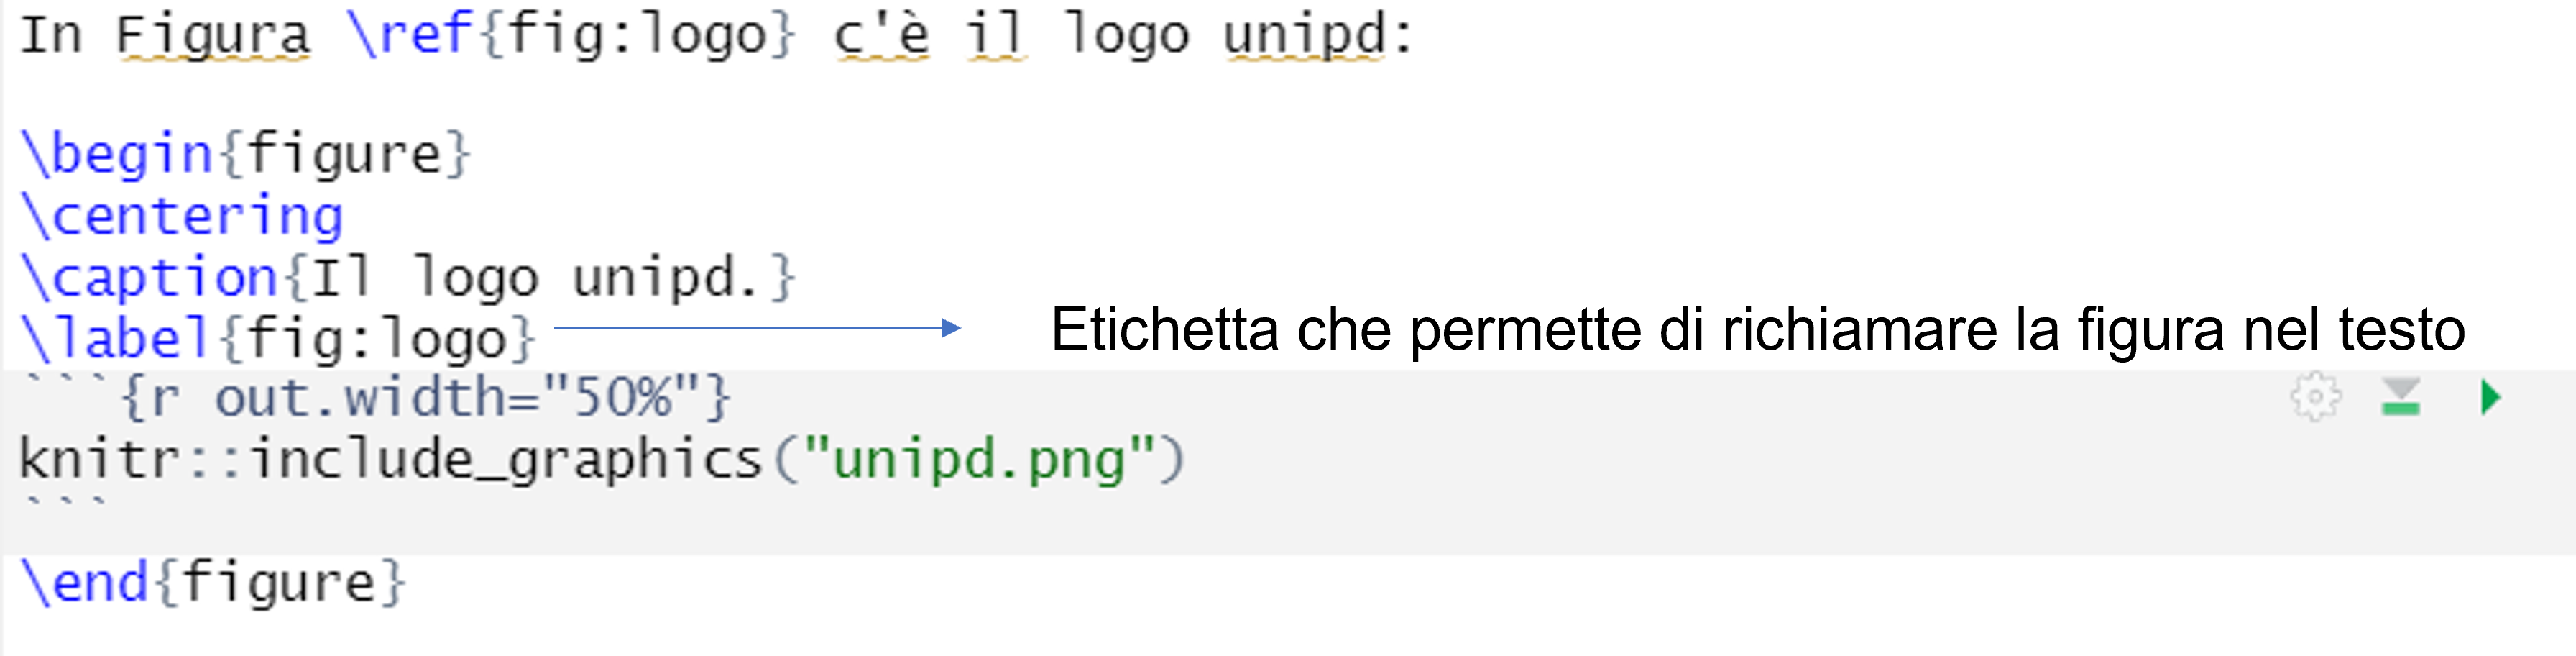
\includegraphics[width=1\linewidth]{img/figure1} \end{center}
\end{frame}

\begin{frame}{Risultato}
\protect\hypertarget{risultato}{}
In Figura \ref{fig:logo} c'è il logo unipd:

\begin{figure}
\centering
\caption{Il logo unipd.}
\label{fig:logo}

\begin{center}
\includegraphics[width=0.5\linewidth]{img/unipd} \end{center}
\end{figure}
\end{frame}

\begin{frame}[fragile]{Le sottofigure}
\protect\hypertarget{le-sottofigure}{}
Bisogna aggiunger allo YAML
\texttt{-\textbackslash{}usepackage\{subcaption\}}

\begin{center}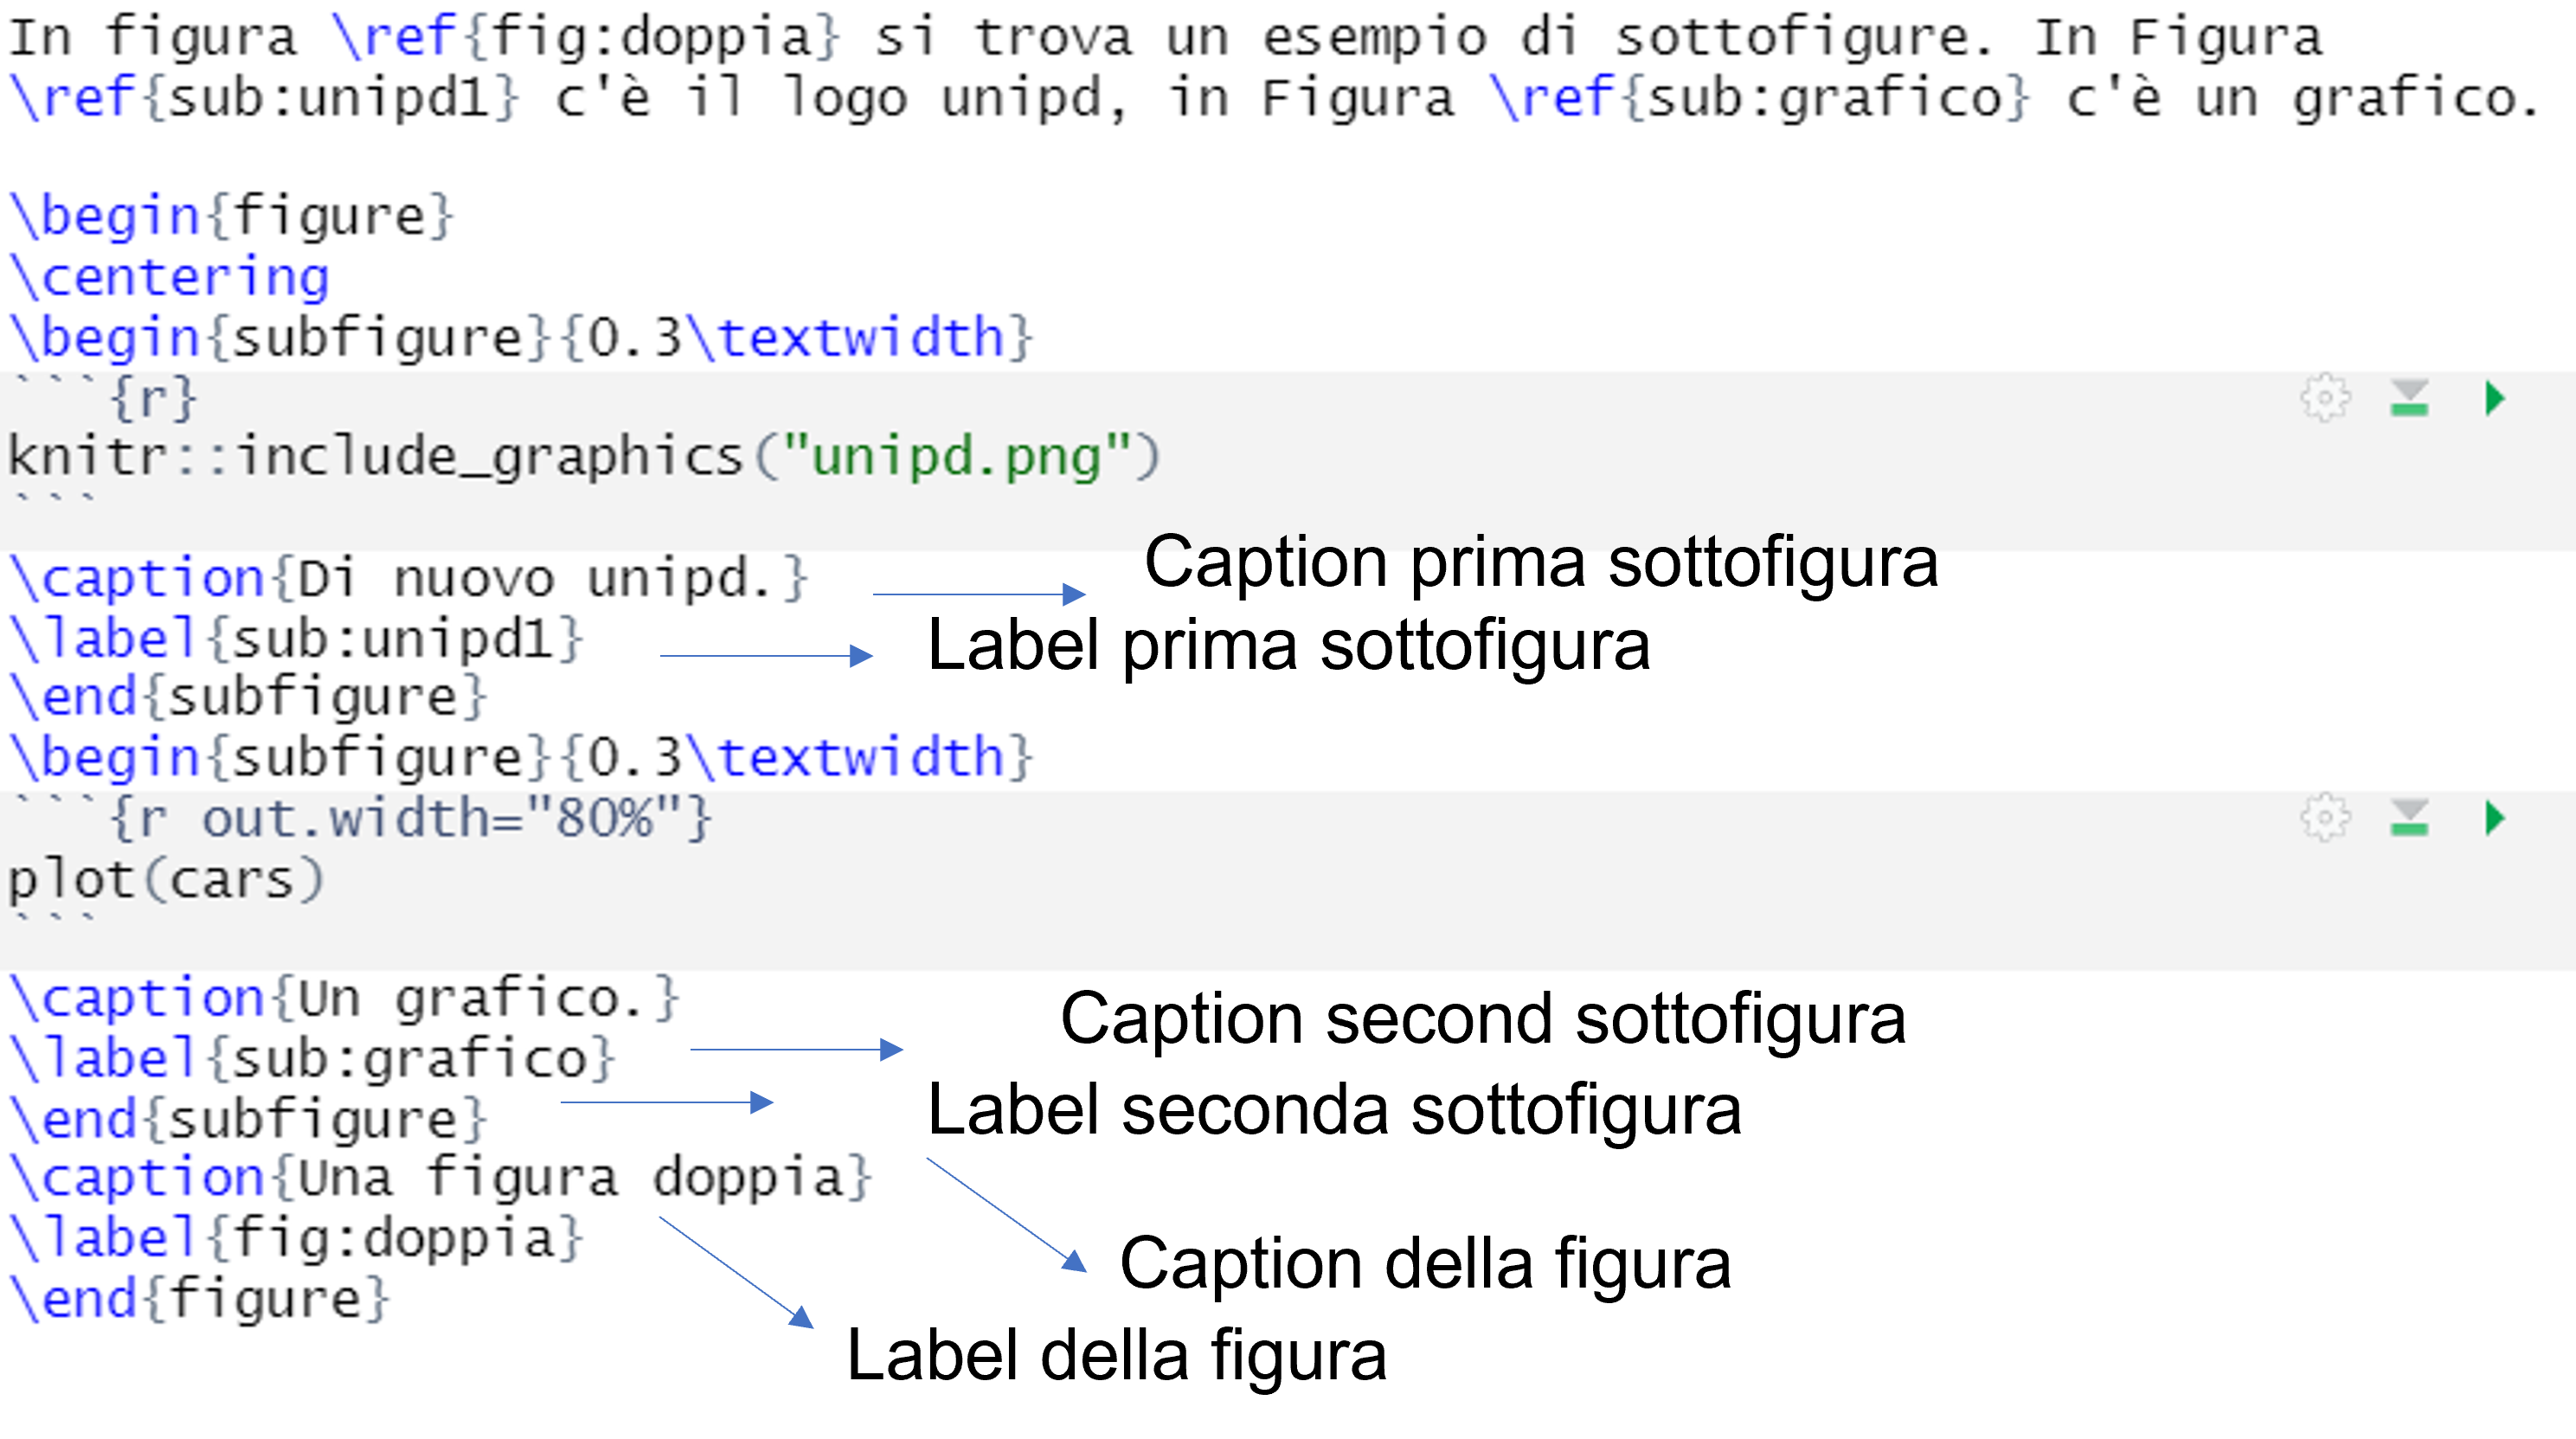
\includegraphics[width=0.9\linewidth]{img/subfigure} \end{center}
\end{frame}

\begin{frame}{}
\protect\hypertarget{section-3}{}
In figura \ref{fig:doppia} si trova un esempio di sottoofigure. In
Figura \ref{sub:unipd1} c'è il logo unipd, in Figura \ref{sub:grafico}
c'è un grafico.

\begin{figure}
\centering
\begin{subfigure}{0.3\textwidth}

\begin{center}
\includegraphics[width=0.5\linewidth]{img/unipd} \end{center}
\caption{Di nuovo unipd.}
\label{sub:unipd1}
\end{subfigure}
\begin{subfigure}{0.3\textwidth}

\begin{center}\includegraphics[width=0.8\linewidth]{03bis-LaTeX-bis_files/figure-beamer/unnamed-chunk-8-1} \end{center}
\caption{Un grafico.}
\label{sub:grafico}
\end{subfigure}
\caption{Una figura doppia}
\label{fig:doppia}
\end{figure}
\end{frame}

\begin{frame}[fragile]{Equazioni}
\protect\hypertarget{equazioni}{}
Funziona il codice che abbiamo visto fino ad adesso (\texttt{\$\$})

Per avere le cross-reference:

\begin{Shaded}
\begin{Highlighting}[]
\NormalTok{\textgreater{} }
\NormalTok{+ In Equazione }\KeywordTok{\textbackslash{}ref}\NormalTok{\{}\ExtensionTok{eq:mean}\NormalTok{\} è riportata la formula per calcolare la media della variabile }\SpecialStringTok{$X$}\NormalTok{:}
\NormalTok{+ }
\NormalTok{+ }\KeywordTok{\textbackslash{}begin}\NormalTok{\{}\ExtensionTok{equation}\NormalTok{\}}\SpecialCharTok{\textbackslash{}label}\SpecialStringTok{\{eq:mean\}}
\SpecialStringTok{+   }\SpecialCharTok{\textbackslash{}bar}\SpecialStringTok{\{X\} = }\SpecialCharTok{\textbackslash{}frac}\SpecialStringTok{\{}\SpecialCharTok{\textbackslash{}sum}\SpecialStringTok{\_\{i=1\}\^{}\{n\} x\_i\}\{n\}}
\SpecialStringTok{+ }\KeywordTok{\textbackslash{}end}\NormalTok{\{}\ExtensionTok{equation}\NormalTok{\}}
\end{Highlighting}
\end{Shaded}

\pause

In Equazione \ref{eq:mean} è riportata la formula per calcolare la media
della variabile \(X\):

\begin{equation}\label{eq:mean}
    \bar{X} = \frac{\sum_{i=1}^{n} x_i}{n}
\end{equation}
\end{frame}

\begin{frame}[fragile]{Tabelle}
\protect\hypertarget{tabelle}{}
\begin{verbatim}
I risultati sono riportati in Tabella \ref{tab:tabella}
\end{verbatim}

\begin{verbatim}
```{r, results='asis'}
print(xtable::xtable(rock[1:7, ], 
                    caption = "Tabella delle rocce", 
                     label = "tab:tabella"), 
      comment = FALSE, 
      caption.placement = "top")
```
\end{verbatim}
\end{frame}

\begin{frame}{}
\protect\hypertarget{section-4}{}
I risultati sono riportati in Tabella \ref{tab:tabella}.

\begin{table}[ht]
\centering
\caption{Tabella delle rocce} 
\label{tab:tabella}
\begin{tabular}{rrrrr}
  \hline
 & area & peri & shape & perm \\ 
  \hline
1 & 4990 & 2791.90 & 0.09 & 6.30 \\ 
  2 & 7002 & 3892.60 & 0.15 & 6.30 \\ 
  3 & 7558 & 3930.66 & 0.18 & 6.30 \\ 
  4 & 7352 & 3869.32 & 0.12 & 6.30 \\ 
  5 & 7943 & 3948.54 & 0.12 & 17.10 \\ 
  6 & 7979 & 4010.15 & 0.17 & 17.10 \\ 
  7 & 9333 & 4345.75 & 0.19 & 17.10 \\ 
   \hline
\end{tabular}
\end{table}
\end{frame}

\begin{frame}[fragile]{Frontespizio}
\protect\hypertarget{frontespizio}{}
Sembra più difficile di quanto non sia:

\footnotesize

\begin{Shaded}
\begin{Highlighting}[]
\NormalTok{\textgreater{} output: }
\NormalTok{+    pdf\_document:}
\NormalTok{+       includes:}
\NormalTok{+         before\_body: titolo.sty}
\NormalTok{+       keep\_tex: yes}
\NormalTok{+       number\_sections: yes}
\NormalTok{+       toc\_depth: 2}
\NormalTok{+ bibliography: biblio.bib}
\NormalTok{+ geometry: margin=1in}
\NormalTok{+ header{-}includes:}
\NormalTok{+   {-} }\BuiltInTok{\textbackslash{}usepackage}\NormalTok{\{}\ExtensionTok{setspace}\NormalTok{\} }
\NormalTok{+   {-} }\BuiltInTok{\textbackslash{}usepackage}\NormalTok{\{}\ExtensionTok{multicol}\NormalTok{\}}
\NormalTok{+   {-} }\BuiltInTok{\textbackslash{}usepackage}\NormalTok{\{}\ExtensionTok{caption}\NormalTok{\}}
\NormalTok{+   {-} }\BuiltInTok{\textbackslash{}usepackage}\NormalTok{[italian]\{}\ExtensionTok{babel}\NormalTok{\}}
\NormalTok{+   {-} }\FunctionTok{\textbackslash{}captionsetup}\NormalTok{\{format=plain, font=small, labelfont=bf\}}
\NormalTok{+   {-} }\BuiltInTok{\textbackslash{}usepackage}\NormalTok{\{}\ExtensionTok{graphicx}\NormalTok{\} }
\NormalTok{+   {-} }\BuiltInTok{\textbackslash{}usepackage}\NormalTok{\{}\ExtensionTok{subcaption}\NormalTok{\}}
\end{Highlighting}
\end{Shaded}
\end{frame}

\begin{frame}[fragile]{}
\protect\hypertarget{section-5}{}
In questo modo si forza \texttt{RMarkdown} a prendere un frontespizio
esterno, creato a parte

Per creare il frontespizio è necessario avere un po' di conoscenze in
\LaTeX

Molto importante: se nel frontespizio usate dei pacchetti (e.g., se
volete aggiungere una figura dovete avere il pacchetto
\texttt{graphicx}) dovete caricarli nello YAML del documento principale

Ho creato
\href{https://drive.google.com/file/d/1O4YgvAZnPJbNMOz0tugz5xf75TTxVvlY/view?usp=sharing}{\textcolor{blue}{titolo.sty}}
per voi, dovete solo modificarlo!
\end{frame}

\begin{frame}[fragile]{Importare la bibliografia}
\protect\hypertarget{importare-la-bibliografia}{}
\begin{Shaded}
\begin{Highlighting}[]
\NormalTok{\textgreater{} output: }
\NormalTok{+    pdf\_document:}
\NormalTok{+       includes:}
\NormalTok{+         before\_body: titolo.sty}
\NormalTok{+ bibliography: biblio.bib \# fatto}
\NormalTok{+ geometry: margin=1in}
\NormalTok{+ header{-}includes:}
\NormalTok{+   {-} }\BuiltInTok{\textbackslash{}usepackage}\NormalTok{\{}\ExtensionTok{setspace}\NormalTok{\} }
\NormalTok{+   {-} }\BuiltInTok{\textbackslash{}usepackage}\NormalTok{\{}\ExtensionTok{multicol}\NormalTok{\}}
\NormalTok{+ [....]}
\end{Highlighting}
\end{Shaded}

Valgono i comandi che abbiamo già visto
\href{https://ottaviae.github.io/CorsoRmarkdown/slides/01\%20-\%20Baby\%20Steps/01-Baby-Steps.html\#38}{\textcolor{blue}{qui}}
\end{frame}

\begin{frame}[fragile]{Cambiare la bibliografia}
\protect\hypertarget{cambiare-la-bibliografia}{}
\small

\begin{Shaded}
\begin{Highlighting}[]
\NormalTok{\textgreater{} output: }
\NormalTok{+    pdf\_document:}
\NormalTok{+       citation\_package: biblatex}
\NormalTok{+       includes:}
\NormalTok{+         before\_body: titolo.sty}
\NormalTok{+       keep\_tex: yes}
\NormalTok{+       number\_sections: yes}
\NormalTok{+       toc\_depth: 2}
\NormalTok{+ bibliography: biblio.bib}
\NormalTok{+ biblio{-}style: numeric}
\NormalTok{+ geometry: margin=1in}
\NormalTok{+ header{-}includes:}
\NormalTok{+   {-} }\BuiltInTok{\textbackslash{}usepackage}\NormalTok{\{}\ExtensionTok{setspace}\NormalTok{\} }
\NormalTok{+   {-} }\BuiltInTok{\textbackslash{}usepackage}\NormalTok{\{}\ExtensionTok{multicol}\NormalTok{\}}
\NormalTok{+ [...]}
\end{Highlighting}
\end{Shaded}

A
\href{https://www.overleaf.com/learn/latex/Biblatex_citation_styles}{\textcolor{blue}{questa pagina}}
trovate tutti i possibili stili di \texttt{biblatex}
\end{frame}

\begin{frame}[fragile]{Stampare la bibliografia}
\protect\hypertarget{stampare-la-bibliografia}{}
Bibliografia ``normale'':

In fondo alla presentazione:

\begin{Shaded}
\begin{Highlighting}[]
\NormalTok{\textgreater{} }\FunctionTok{\textbackslash{}clearpage}\NormalTok{ \# Stampa su una pagina nuova}
\NormalTok{+ }
\NormalTok{+ \# Bibliografia}
\end{Highlighting}
\end{Shaded}

\pause

Bibliografia \texttt{biblatex}:

\begin{Shaded}
\begin{Highlighting}[]
\NormalTok{\textgreater{} }\FunctionTok{\textbackslash{}clearpage}\NormalTok{ \# Stampa su una pagina nuova}
\NormalTok{+ }
\NormalTok{+ \# Bibliografia}
\end{Highlighting}
\end{Shaded}

\pause

Problema: Non appare la bibliografia nell'indice
\end{frame}

\begin{frame}[fragile]{Your turn!}
\protect\hypertarget{your-turn}{}
\small

\begin{itemize}
\item
  Usando
  \href{https://drive.google.com/file/d/1O4YgvAZnPJbNMOz0tugz5xf75TTxVvlY/view?usp=sharing}{\textcolor{blue}{titolo.sty}}
  mettete il logo del vostro dataset
\item
  Cambiate il titolo, autore, corso e quello che volete a seconda della
  vostra fantasia
\item
  Mettete tre Titoli (Header 1, e.g., ``Introduzione'', ``Metodo'',
  ``Risultati'') (se volete potete mettere del testo)
\item
  Inserite una figura con tre sottofigure (due foto e il grafico del
  vostro dataset) con rispettive cross-reference nel testo
\item
  Inserite un'equazione (potete usare quella della standardizzazione)
\item
  Inserite una tabella descrittiva del vostro dataset con
  cross-reference nel testo
\item
  Importate la bibliografia
\end{itemize}

\begin{center}
ADAVANCED
\end{center}

\begin{itemize}
\item
  Integrate l'equazione con i numeri reali del vostro dataset
\item
  Inserite una tabella con i risultati del modello del vostro dataset
  (ovviamente con cross-reference)
\item
  Inserite una tabella con model comparison
  (\texttt{m0\ =\ lm(y\ \textasciitilde{}\ x,\ data\ =\ vostro\_datase})
\end{itemize}
\end{frame}

\hypertarget{presentazioni}{%
\section{Presentazioni}\label{presentazioni}}

\begin{frame}{Lo YAML}
\protect\hypertarget{lo-yaml-1}{}
\begin{center}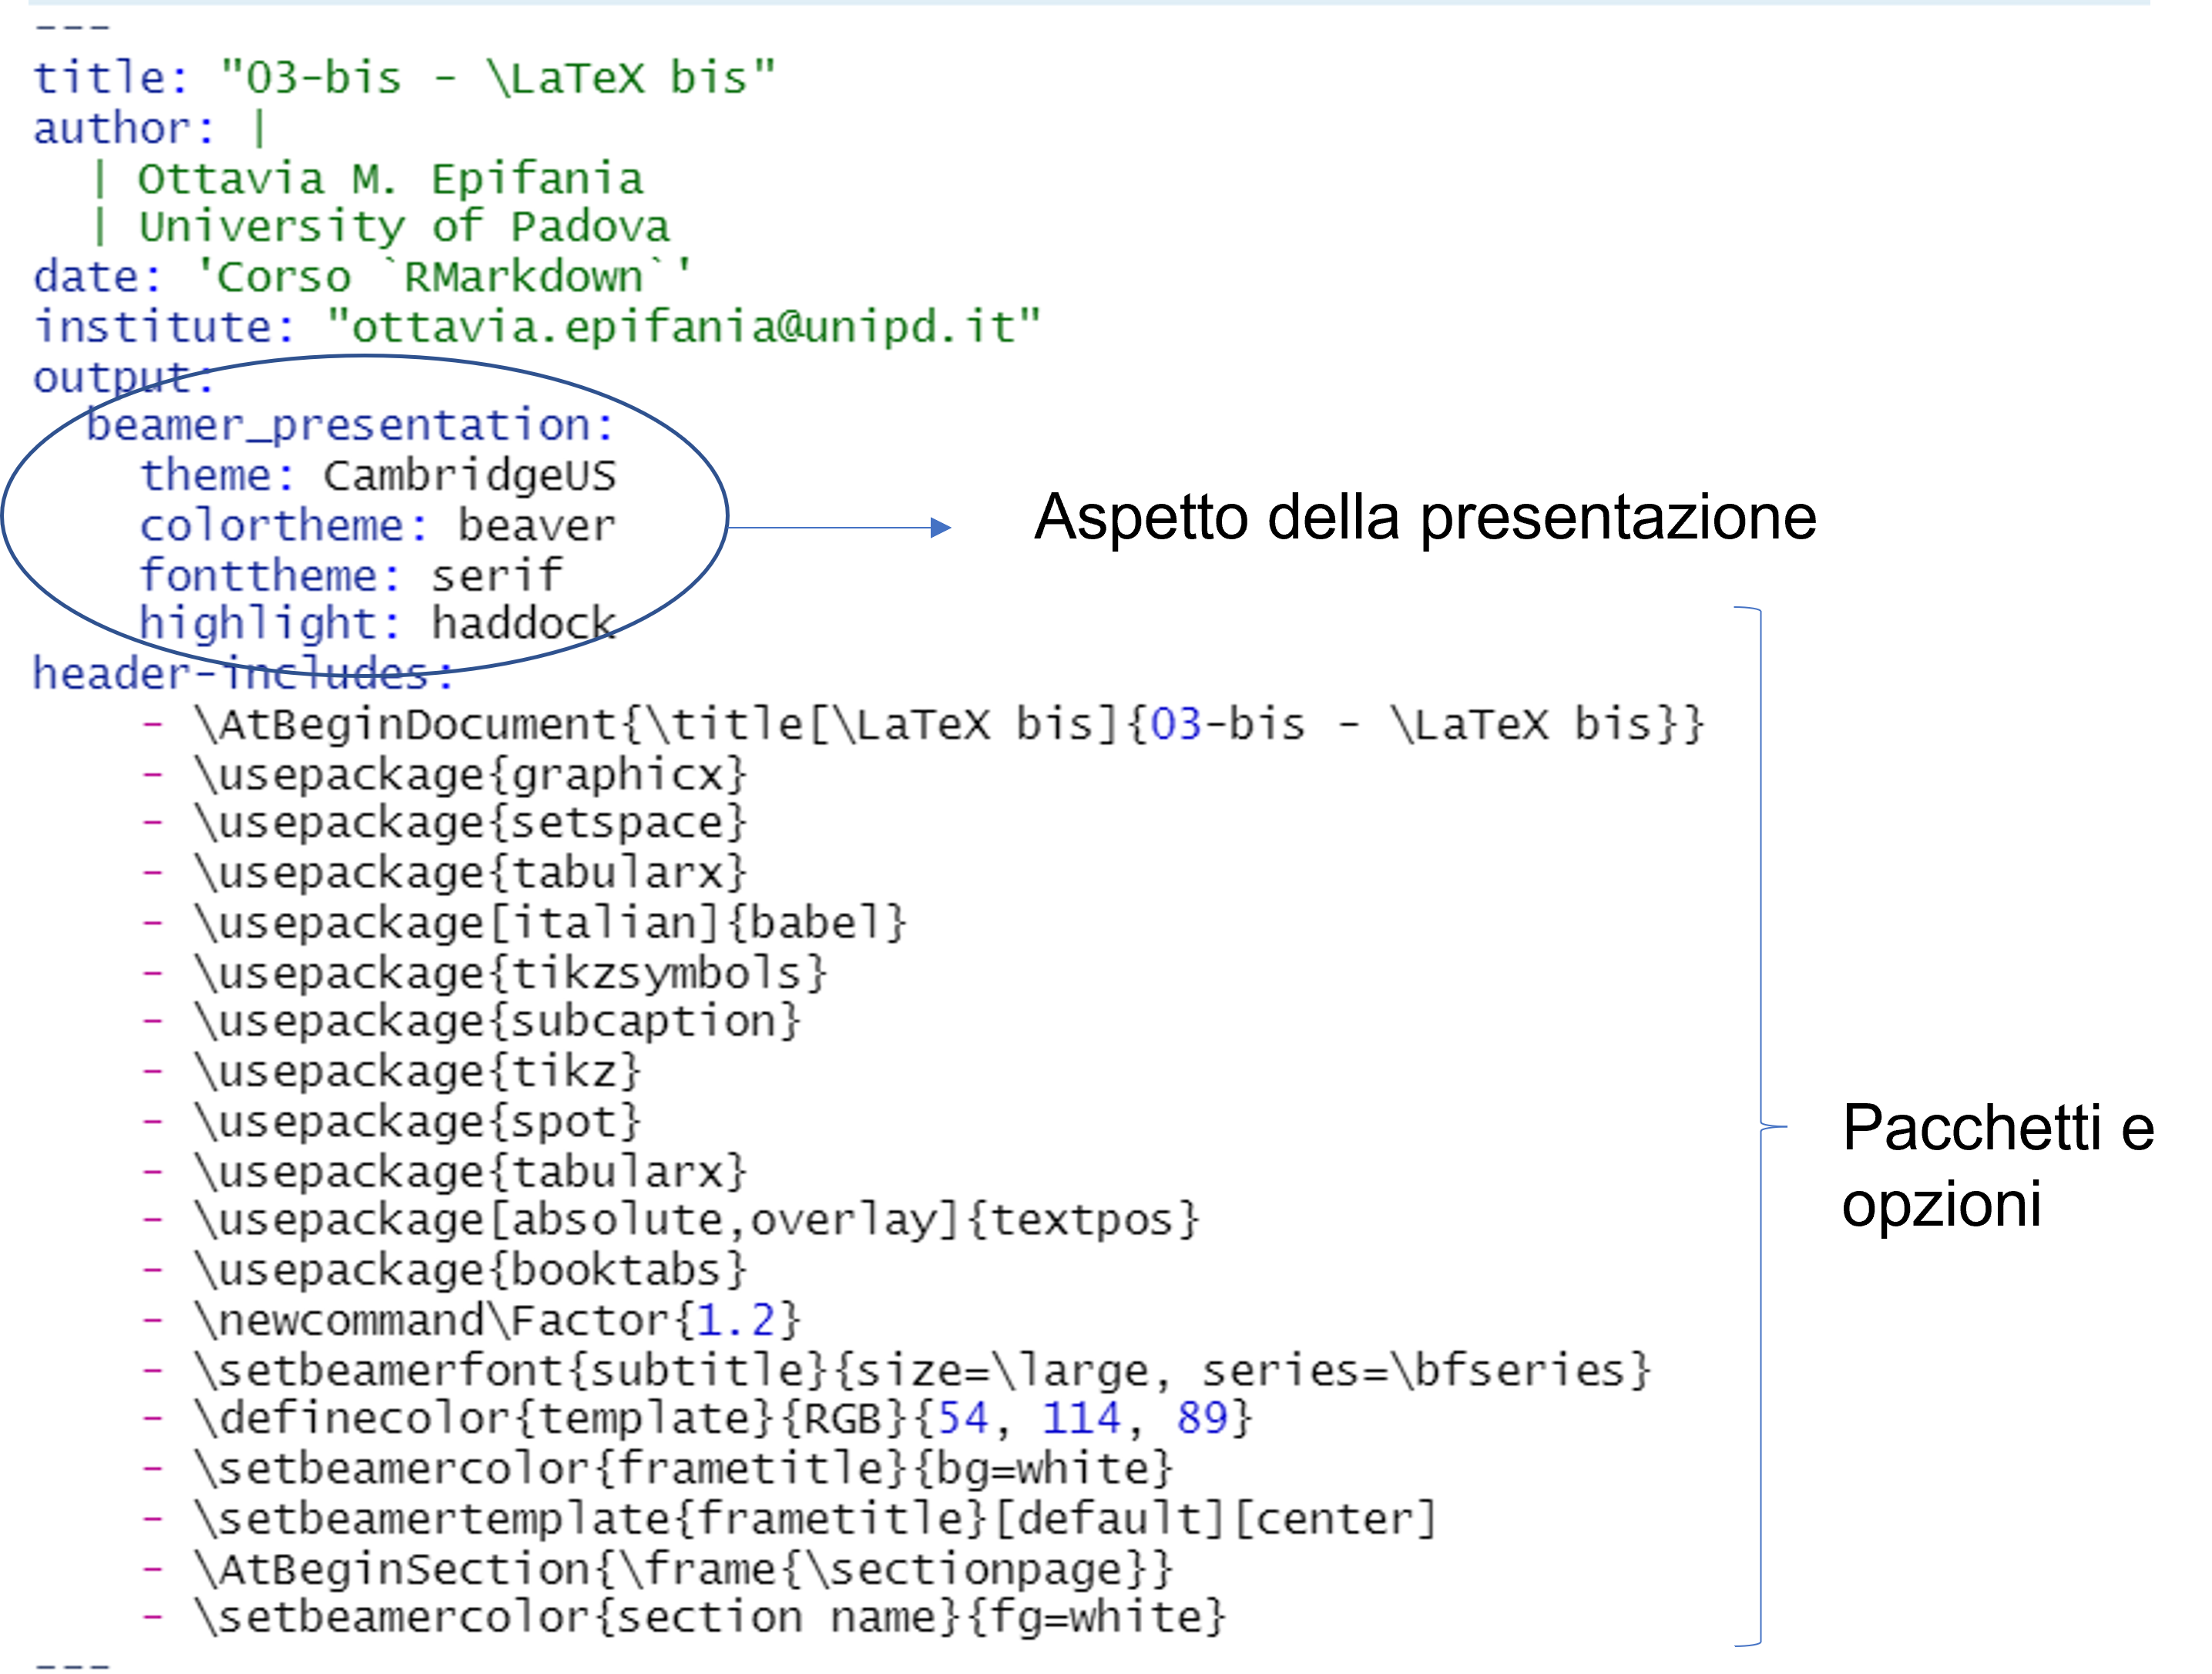
\includegraphics[width=0.8\linewidth]{img/yaml1} \end{center}
\end{frame}

\begin{frame}[fragile]{}
\protect\hypertarget{section-6}{}
Si può scegliere combinazione di \texttt{theme}, \texttt{colortheme},
\texttt{fonttheme} e \texttt{highlight}.

A
\href{https://deic.uab.cat/~iblanes/beamer_gallery/}{\textcolor{blue}{questa pagina}}
sono disponibili tutti i possibili temi per la vostra presentazione

\texttt{highlight} è la formattazione del vostro codice, a cui potete
accedere cliccando sulla rotellina accanto a \texttt{knit}
\(\rightarrow\) Output Options
\end{frame}

\begin{frame}[fragile]{Colonne}
\protect\hypertarget{colonne}{}
Mi raccomando: \texttt{-\ \textbackslash{}usepackage\{multicol\}} deve
essere nello YAML:

\small

\begin{Shaded}
\begin{Highlighting}[]
\NormalTok{\textgreater{} }
\NormalTok{+ }\KeywordTok{\textbackslash{}begin}\NormalTok{\{}\ExtensionTok{columns}\NormalTok{\} }\CommentTok{\% L\textquotesingle{}ambiente colonna}
\NormalTok{+ }\KeywordTok{\textbackslash{}begin}\NormalTok{\{}\ExtensionTok{column}\NormalTok{\}\{0.50}\FunctionTok{\textbackslash{}textwidth}\NormalTok{\}}
\NormalTok{+ Testo nella prima colonna}
\NormalTok{+ }\KeywordTok{\textbackslash{}end}\NormalTok{\{}\ExtensionTok{column}\NormalTok{\}}
\NormalTok{+ }
\NormalTok{+ }\KeywordTok{\textbackslash{}begin}\NormalTok{\{}\ExtensionTok{column}\NormalTok{\}\{0.50}\FunctionTok{\textbackslash{}textwidth}\NormalTok{\}}
\NormalTok{+ Testo nella seconda colonna}
\NormalTok{+ }\KeywordTok{\textbackslash{}end}\NormalTok{\{}\ExtensionTok{column}\NormalTok{\}}
\NormalTok{+ }
\NormalTok{+ }\KeywordTok{\textbackslash{}end}\NormalTok{\{}\ExtensionTok{columns}\NormalTok{\}}
\end{Highlighting}
\end{Shaded}

\pause

\normalsize

\begin{columns} % L'ambiente colonna
\begin{column}{0.50\textwidth}
Testo nella prima colonna
\end{column}

\begin{column}{0.50\textwidth}
Testo nella seconda colonna
\end{column}

\end{columns}

PS: si possono mettere anche più di due colonne
\end{frame}

\begin{frame}[fragile]{Testo incrementale}
\protect\hypertarget{testo-incrementale}{}
Avete visto che in alcune mie slide il testo appare in modo
incrementale. Questo effetto si può ottenere in due modi, entrambi
basati su \LaTeX:

\texttt{\textbackslash{}pause}

Questo è il comando più semplice, si mette davanti al contenuto che si
vuole ``bloccare''

\pause

\vspace{3mm}

\begin{columns}
\begin{column}{.50\linewidth}



Testo che appare subito

\verb=\pause=

Testo che appare dopo la pausa

\end{column}

\pause 

\vspace{3mm}

\begin{column}{.50\linewidth}

Testo che appare subito

\pause 

Testo che appare dopo la pausa


\end{column}
\end{columns}
\end{frame}

\begin{frame}[fragile]{}
\protect\hypertarget{section-7}{}
\texttt{\textbackslash{}onslide\textless{}i-n\textgreater{}}

Dove \(i\) è la prima slide su cui il contenuto deve apparire, \(n\) è
l'ultima slide su cui il contenuto appare (\(n\)) può essere omesso.

\verb=\onslide<2-> Appare sulla seconda slide e rimane fino alla fine=

\verb=\onslide<3-3> Appare alla terza slide e sparisce alla terza=

\verb=\onslide<4-> Appare sull'ultima slide=

\onslide<2-> Appare sulla seconda slide e rimane fino alla fine

\onslide<3-3> Appare alla terza slide e sparisce alla terza

\onslide<4-> Appare sull'ultima slide
\end{frame}

\begin{frame}{Your turn!}
\protect\hypertarget{your-turn-1}{}
\begin{itemize}
\item
  Create una slide con due colonne
\item
  Fate apparire una colonna alla volta
\item
  Nella prima colonna: un'immagine
\item
  Nella seconda colonna: testo
\end{itemize}
\end{frame}

\begin{frame}{Blocchi di testo}
\protect\hypertarget{blocchi-di-testo}{}
\begin{block}{Il testo}

Viene racchiuso in blocchi che lo mettono in risalto

\end{block}

\pause

\vspace{3mm}

\begin{exampleblock}{Blocchi di esempio}

Dove il titolo è in verde e a seconda del tema scelto anche la sfumatura esterna del blocco stesso

\end{exampleblock}

\pause

\vspace{3mm}

\begin{alertblock}{Blocchi di Warning}

Dove il titolo è in rosso e a seconda del tema scelto anche la sfumatura esterna del blocco stesso

\end{alertblock}
\end{frame}

\begin{frame}[fragile]{}
\protect\hypertarget{section-8}{}
\footnotesize

\begin{Shaded}
\begin{Highlighting}[]
\NormalTok{\textgreater{} }\KeywordTok{\textbackslash{}begin}\NormalTok{\{}\ExtensionTok{block}\NormalTok{\}\{Il testo\}}
\NormalTok{+ }
\NormalTok{+ Viene racchiuso in blocchi che lo mettono in risalto}
\NormalTok{+ }
\NormalTok{+ }\KeywordTok{\textbackslash{}end}\NormalTok{\{}\ExtensionTok{block}\NormalTok{\}}
\NormalTok{+ }
\NormalTok{+ }\FunctionTok{\textbackslash{}pause}
\NormalTok{+ }
\NormalTok{+ }\KeywordTok{\textbackslash{}begin}\NormalTok{\{}\ExtensionTok{exampleblock}\NormalTok{\}\{Blocchi di esempio\}}
\NormalTok{+ }
\NormalTok{+ Dove il titolo è in verde e a seconda del tema scelto anche la sfumatura esterna del blocco stesso}
\NormalTok{+ }
\NormalTok{+ }\KeywordTok{\textbackslash{}end}\NormalTok{\{}\ExtensionTok{exampleblock}\NormalTok{\}}
\NormalTok{+ }
\NormalTok{+ }\FunctionTok{\textbackslash{}pause}
\NormalTok{+ }
\NormalTok{+ }\KeywordTok{\textbackslash{}begin}\NormalTok{\{}\ExtensionTok{alertblock}\NormalTok{\}\{Blocchi di Warning\}}
\NormalTok{+ }
\NormalTok{+ Dove il titolo è in rosso e a seconda del tema scelto anche la sfumatura esterna del blocco stesso}
\NormalTok{+ }
\NormalTok{+ }\KeywordTok{\textbackslash{}end}\NormalTok{\{}\ExtensionTok{alertblock}\NormalTok{\}}
\end{Highlighting}
\end{Shaded}
\end{frame}

\begin{frame}{Your turn!}
\protect\hypertarget{your-turn-2}{}
\begin{itemize}
\item
  Create una slide con due colonne, nella prima colonna testo, nella
  seconda colonna testo e una figura
\item
  Far apparire la seconda colonna, il suo testo e la sua figura uno alla
  volta
\item
  Create una slide con 3 blocchi
\end{itemize}

\begin{center}
ADVANCED
\end{center}

\begin{itemize}
\tightlist
\item
  Fate apparire i blocchi così:

  \begin{itemize}
  \tightlist
  \item
    il terzo blocco sulla prima slide e rimane fino alla fine
  \item
    il secondo blocco compare e scompare alla seconda slide
  \item
    il primo blocco appare e rimane sull'ultima slide
  \end{itemize}
\end{itemize}
\end{frame}

\end{document}
